\newcommand{\pnl}{P\&L}

\begin{idea}
	Convexity and non-uniqueness are different things. If convex problem has large eps-null space, i.e. large flat area around the optimum, then
	\begin{itemize}
		\item it is bad for consistency of solver: using different methods will give you different argmaxes;
		\item it is good in practice, since this allows for a secondary objective
	\end{itemize}
\end{idea}

\begin{idea}
	$\max \mu^T w - \gamma w^T \Sigma w $ does not make sense because you are comparing terms that have $units$ and $units^2$, but $\max \mu^T w - \gamma' \sqrt{w^T \Sigma w}$ makes sense. By sweeping $\gamma$ and $\gamma'$ we get exactly same efficient frontier. It is also better \underline{computationally} (more modern)!
	\begin{proof}
		When you have a bi-objective optimization problem and apply monotonic transformation to either or both and then take sum you get same efficient frontier.
	\end{proof}
\end{idea}

\begin{idea}
	If you solve LeastSquare problem within x ms, the cost of solving a convex problem with the same structure is about 10-100 times more, maybe 20. Because interior point method does about 20 iterations.
\end{idea}

\begin{idea}
	Risk neutrality. Instead of 
	\begin{align}
		m^T w = 0
	\end{align}

	we should do
	
	\begin{align}
		m^T \Sigma w = 0
	\end{align}

	because this corresponds to orthogonality of market portfolio \pnl  ($M = m^T r$) and portfolio \pnl ($R = w^T r$).
	
\end{idea}

\begin{idea}
	\textrm{V@R} is not convex, but \textrm{cV@R} is. And it turns out you don't want to do but \textrm{V@R} as it is not a:
	\begin{itemize}
		\item \textrm{V@R} -- you want prob of your drawdown exceeding 10\% is no more than 5\%.
		\item \textrm{cV@R} -- I want conditional expectation of the drawdown to be less than this given that is greater than 10\%. 
	\end{itemize}
\end{idea}

\begin{idea}
	If you can add a lot of constraints and they don't change result (objective value) too much, then add as many and tighten up. It is like insurance for which you hardly pay anything, but if bad event happens you are in a much better shape.
\end{idea}

\begin{idea}
	$w \in \Rplus^n \Leftrightarrow \norm{w}_1 \le 1$, i.e. non negativity is constrained on leverage.
\end{idea}

\begin{idea}
	Non-negativity constraint, l1-norm and alpha uncertainty generate sparse solutions.
	
	If something is small, in l1 you pay small, but in l2 you pay very small. If you have something already small, for l2 there is no particular motivation to make it zero. But for l2 the \underline{marginal advantage} of making it smaller keeps up.
	
	And for non-negativity, that's like having infinite value to the left of zero. As long as I have non-zero negative slope from right at zero, I'll have sparsity also. E.g. $max(0, (x+1)^2 - 1)$ or $max(0, x)$. See \autoref{fig:sparsepenalties} 
	
	\begin{figure}[h]
		\centering
		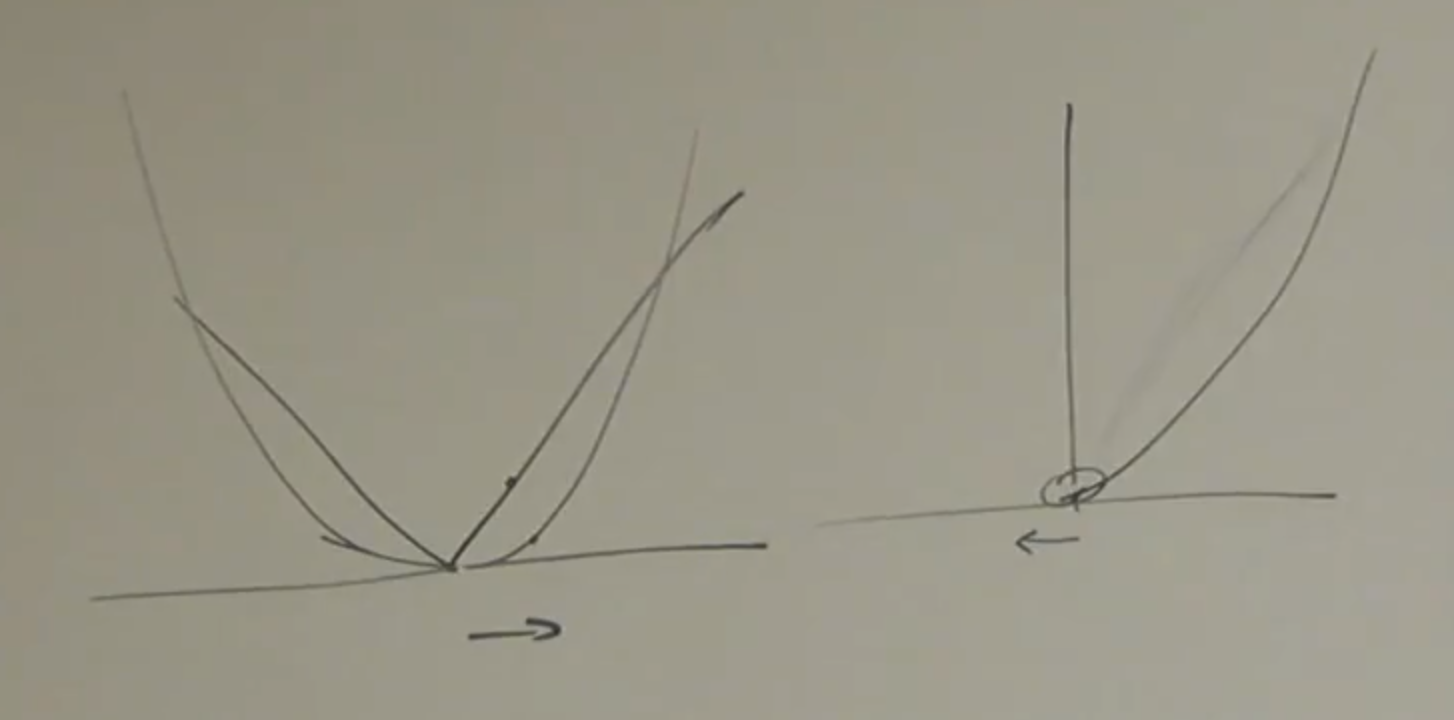
\includegraphics[width=0.7\linewidth]{img/sparse_penalties}
		\caption{}
		\label{fig:sparsepenalties}
	\end{figure}
	
\end{idea}

\begin{idea}
	Every reasonable transaction cost is convex
\end{idea}

\begin{idea}
	$k$-day liquidation cost: $k\phi^{tc}(w/k)$. Because of convexity, you need to trade evenly. If part of $\phi^{tc}$ is linear (spread) cost, then this will involve $l1$ penalty on positions and we'll start seeing zero positions, because these stocks are too illiquid to hold and get out when necessary...
\end{idea}

\begin{idea}
	Doing optimization vs doing simulation are different things: people who do simulation certainly care whether impact has power $3/2$ or $2$. People who do optimization just think of it as "something that discourages large trades", while spread cost term as "something that discourages small trades".
\end{idea}

\begin{idea}
	Introducing variables for exposures $f = F^t x$ should \underline{always} be done:
	\begin{itemize}
		\item it reduces computational complexity from $\bigO(n^3)$ to $\bigO(n k^2)$;
		\item now we can put constraints on factor exposures.
	\end{itemize}
\end{idea}

\begin{idea}
	Fitting low-rank + diagonal model is not a convex problem but it is perfectly solvable.
\end{idea}

\begin{idea}
	It is a very good idea to add constraints on exposures, because it is a better risk control. The quadratics is a BIG LIE. If you look at covariance matrix, there are only a few significant eigenvalues and it says that there are 3600 directions with zero risk! Constrain those directions!!!
\end{idea}

\begin{idea}
	Forecast uncertainty. Let's say instead of point estimate vector $mu$ we are given intervals $\mu^{low} \le \mu \le \mu^{high}$. Introduce \underline{vectors}
	\begin{align}
		\bar{\mu} &= \frac{\mu^{low}+\mu^{high}}{2} \\ 
		\bar{\mu} &= \frac{\mu^{high}-\mu^{low}}{2} (\text{vector of uncertainty})
	\end{align}
	Then worst-case $\mu$ is easy to get analytically
	\begin{align}
		\min_{\mu^{low} \le \mu \le \mu^{high}} \mu^T h = \bar{\mu} - \underbrace{\sigma^T |h|}_{\text{weighted l1-norm}}
	\end{align}

The second term is alpha-uncertainty risk. L1-norm weighted by alpha uncertainties.

\end{idea}

\begin{idea}
	How to get covariance scenarios?
	\begin{itemize}
		\item manually (labeled)
		\item perturb nominal cov matrices in a reasonable way (remember to adjust corr matrix as it may stop being corr matrix: svd and replace negative eigenvalues, or add identity or project onto $S_+$ or closest matrix in $S_+$)
	\end{itemize}
\end{idea}